\documentclass[tikz,border=4pt]{standalone}
\usepackage{pgfplots}
\pgfplotsset{compat=1.16}
\pgfplotsset{
  bode/.style={
    width=6.4cm, height=4.4cm, xmin=0.01, xmax=100,
    grid=both, major grid style={gray!55}, minor grid style={gray!20},
    tick label style={font=\footnotesize}, label style={font=\small},
    title style={font=\small}, xlabel={$\omega/\omega_u$},
  },
  bode mag/.style={bode, ymin=-50, ymax=50, ytick={-40,-20,0,20,40},
    ylabel={$|H|_{\mathrm{dB}}$}, title={Modulo}},
  bode fase/.style={bode, ymin=-100, ymax=100, ytick={-90,-45,0,45,90},
    ylabel={$\varphi$ [$^\circ$]}, title={Fase}},
}
\begin{document}
% Integratore ideale: H(j w) = -1/(j w R C) = j wu/w,  wu = 1/(RC),  x = w/wu
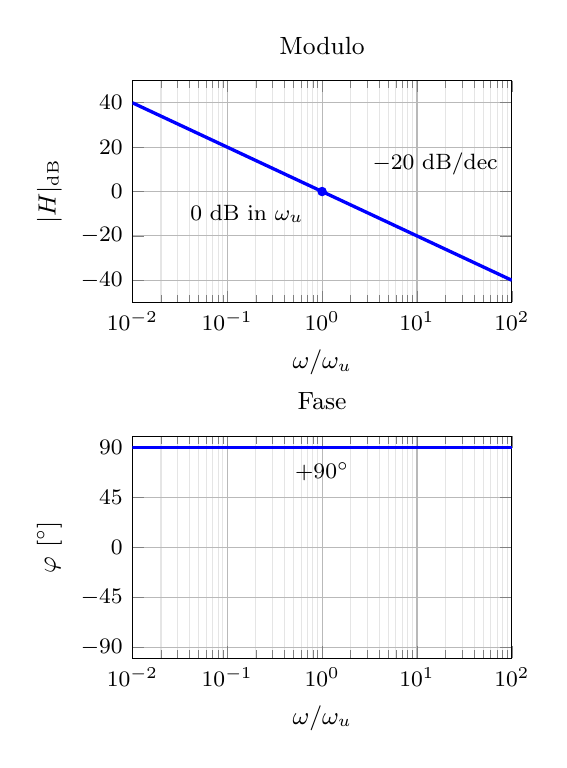
\begin{tikzpicture}
% ---------- modulo ----------
\begin{semilogxaxis}[bode mag, name=mag]
  \addplot[blue, very thick] coordinates {(0.01,40) (100,-40)};
  \addplot[only marks, mark=*, mark size=1.5pt, blue] coordinates {(1,0)};
  \node[anchor=north east, font=\footnotesize] at (axis cs:0.8,-1.5) {$0$ dB in $\omega_u$};
  \node[anchor=north east, font=\footnotesize] at (axis cs:90,22) {$-20$ dB/dec};
\end{semilogxaxis}
% ---------- fase ----------
\begin{semilogxaxis}[bode fase, at={(mag.south west)}, yshift=-1.7cm, anchor=north west]
  \addplot[blue, very thick] coordinates {(0.01,90) (100,90)};
  \node[anchor=north, font=\footnotesize] at (axis cs:1,85) {$+90^\circ$};
\end{semilogxaxis}
\end{tikzpicture}
\end{document}
